\section{Xilinx PCIe Core}
The PCIe Engine is based on the interface of the Virtex-7 FPGA Gen3 Integrated Block for PCI Express v3.0 \cite{pg023}. This core is using a PCIe hard block in Virtex-7 FPGAs. The hard block is equipped with an AXI4-Stream interface.
\subsection{Xilinx AXI4-Stream interface}
The interface has the advantage that it has two separate bidirectional AXI4-Stream interfaces. The two interfaces are the requester interface, with which the FPGA issues the requests and the PC replies, and the completer interface where the PC takes initiative.
\begin{table}[H]
	\centering
	\begin{tabularx}{\textwidth}{|l|X|l|}
	\hline
	  \textbf{bus} & \textbf{Description} &\textbf{Direction}\\
	\hline
	\texttt{axis\_rq} & \textbf{R}equester re\textbf{Q}uest. This interface is used for DMA, the FPGA takes the initiative to write to this AXI4-Stream interface and the PC has to answer. &FPGA $\rightarrow$ PC\\
	\hline
	\texttt{axis\_rc} & \textbf{R}equester \textbf{C}ompleter. This interface is used for DMA reads (from PC memory to FPGA), this interface also receives a reply message from the PC after a DMA write.&PC $\rightarrow$ FPGA\\
	\hline
	\texttt{axis\_cq} & \textbf{C}ompleter re\textbf{Q}uest. This interface is used to write the DMA descriptors as well as some other registers. & PC $\rightarrow$ FPGA\\
	\hline
	\texttt{axis\_cc} & \textbf{C}ompleter \textbf{C}ompleter. This interface is used as a reply inteface for register reads, as well as a reply header for a register write. & FPGA $\rightarrow$ PC\\
	\hline
	
	\end{tabularx}
	\caption{AXI4-Stream streams}\label{tab:axi_streams}
\end{table}
\subsection{Configuration of the core}
The Xilinx PCIe core is configured as a PCI express Gen3 (8.0GT/s) core with 8 lanes and the Physical Function (PF0) max payload size is set to 1024 bytes. AXI-ST Frame Straddle is disabled and the client tag is enabled. All other options are set to default, the reference clock frequency is 100MHz and the only option for the AXI4-Stream interface is 256 bit at 250MHz, see Figure~\ref{fig:pcie_core_config1} to \ref{fig:pcie_core_config11}.
\newpage

\begin{figure}[H]
\centering
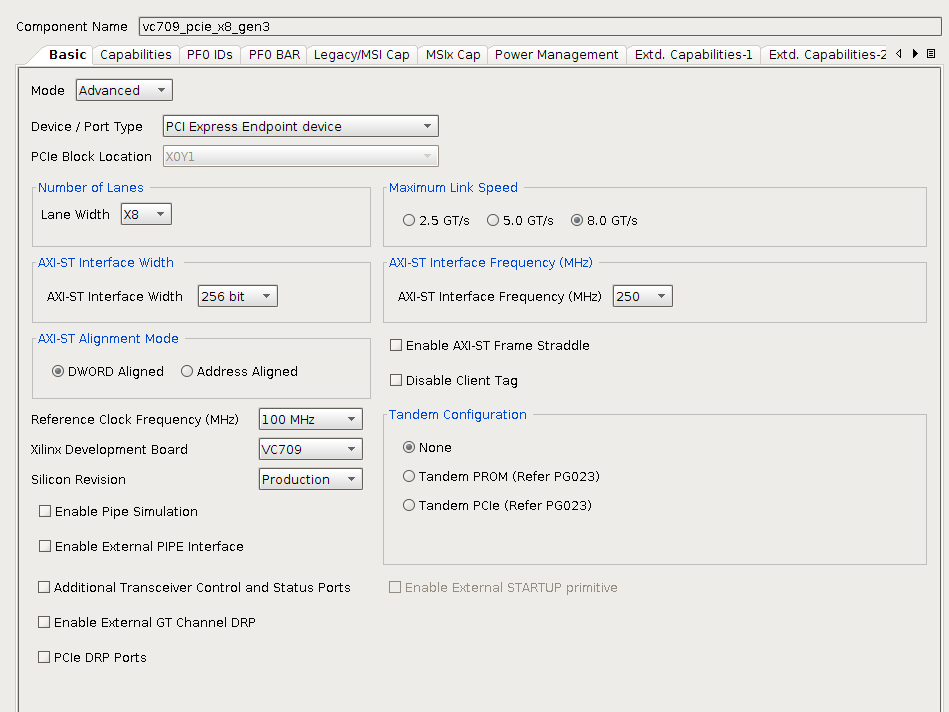
\includegraphics[width=0.75\textwidth]{pictures/pcie_core_basic.png}
\caption{PCIe core configuration in Vivado [Basic]}
\label{fig:pcie_core_config1}
\end{figure}

\begin{figure}[H]
\centering
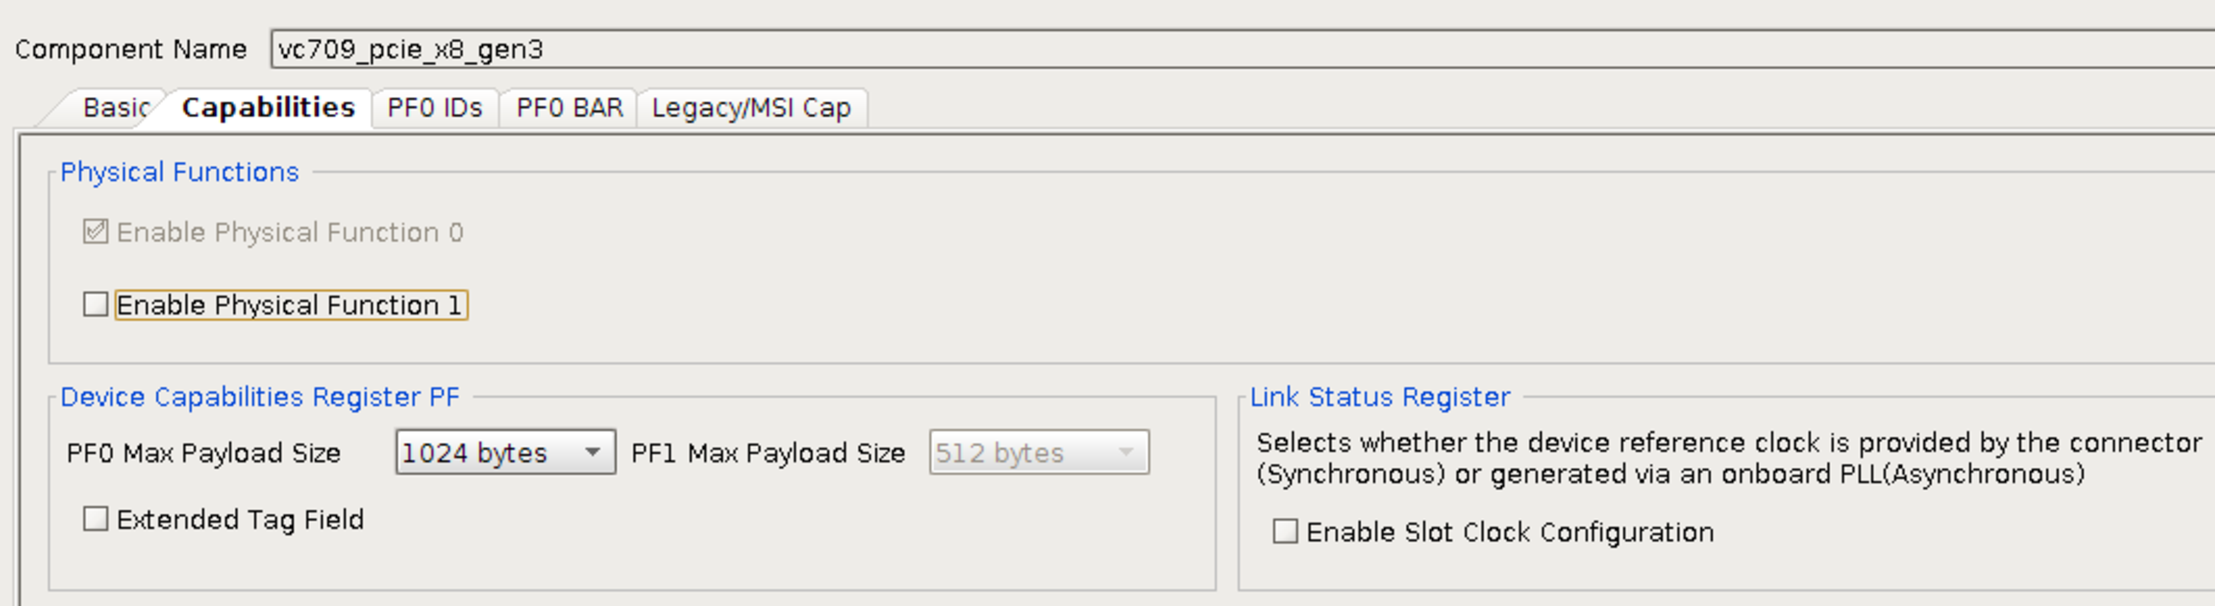
\includegraphics[width=0.75\textwidth]{pictures/pcie_core_config2.pdf}
\caption{PCIe core configuration in Vivado [Capabilities]}
\label{fig:pcie_core_config2}
\end{figure}

\begin{figure}[H]
\centering
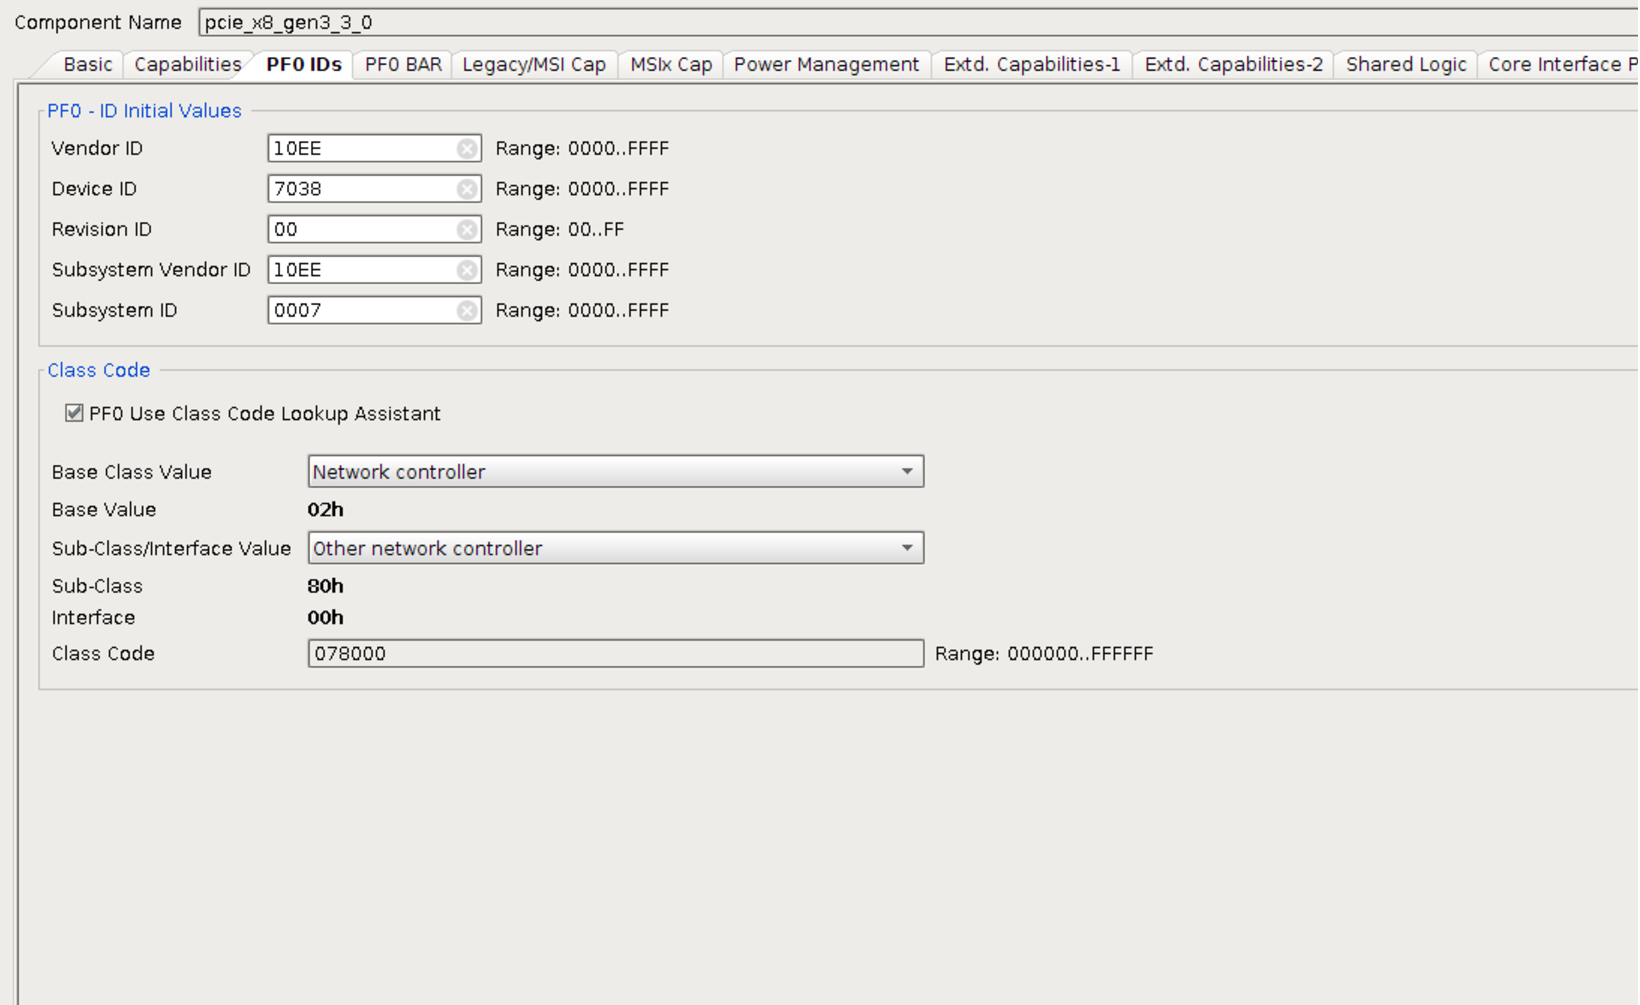
\includegraphics[width=0.75\textwidth]{pictures/pcie_core_config3.pdf}
\caption{PCIe core configuration in Vivado [PF0 IDs]}
\label{fig:pcie_core_config3}
\end{figure}
\newpage
\begin{figure}[H]
\centering
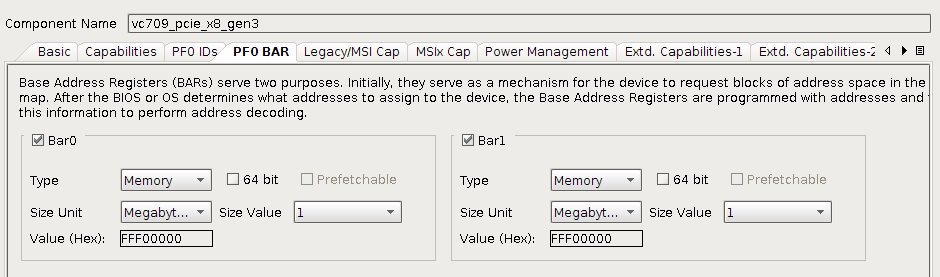
\includegraphics[width=0.75\textwidth]{pictures/pcie_core_pf0_bar.png}
\caption{PCIe core configuration in Vivado [PF0 BAR]}
\label{fig:pcie_core_config4}
\end{figure}

\begin{figure}[H]
\centering
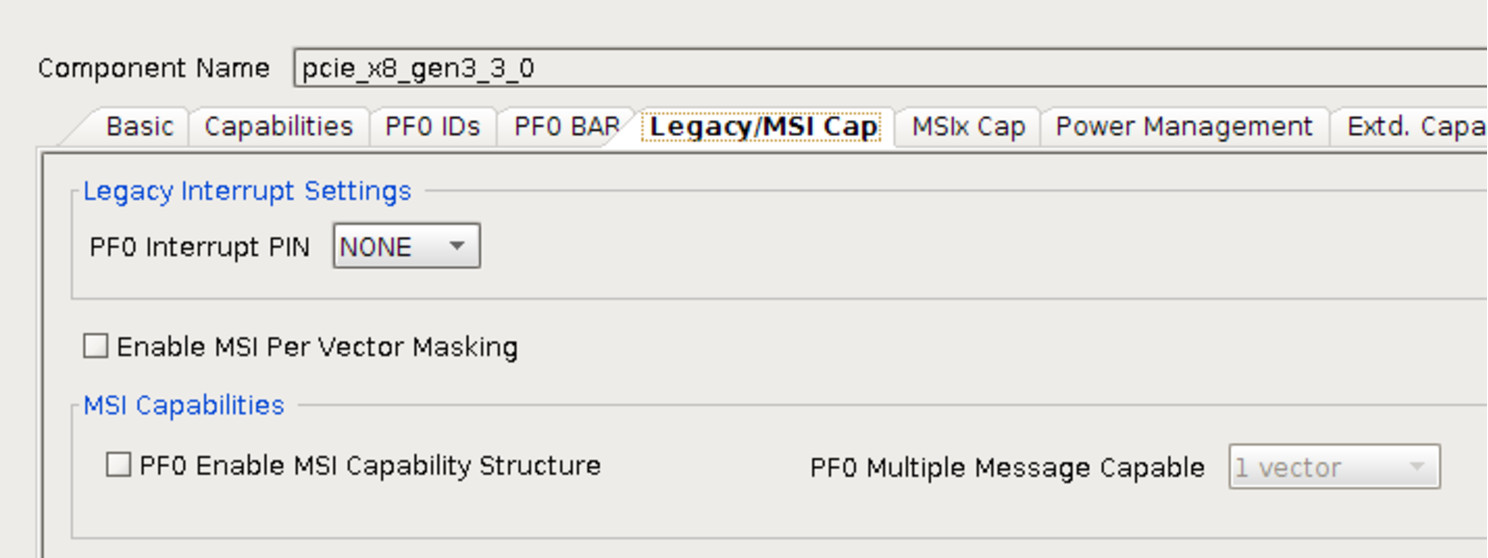
\includegraphics[width=0.75\textwidth]{pictures/pcie_core_config5.pdf}
\caption{PCIe core configuration in Vivado [Legacy/MSI Cap]}
\label{fig:pcie_core_config5}
\end{figure}

\begin{figure}[H]
\centering
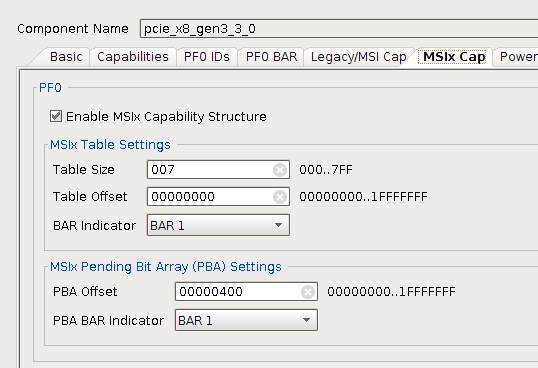
\includegraphics[width=0.75\textwidth]{pictures/pcie_core_msix.png}
\caption{PCIe core configuration in Vivado [MSIx]}
\label{fig:pcie_core_config6}
\end{figure}
\newpage

\begin{figure}[H]
\centering
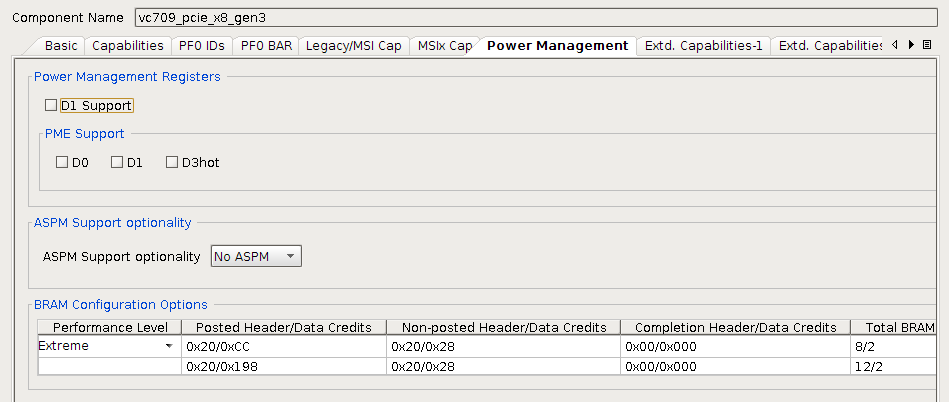
\includegraphics[width=0.75\textwidth]{pictures/pcie_core_pwr.png}
\caption{PCIe core configuration in Vivado [Power Management]}
\label{fig:pcie_core_config7}
\end{figure}

\begin{figure}[H]
\centering
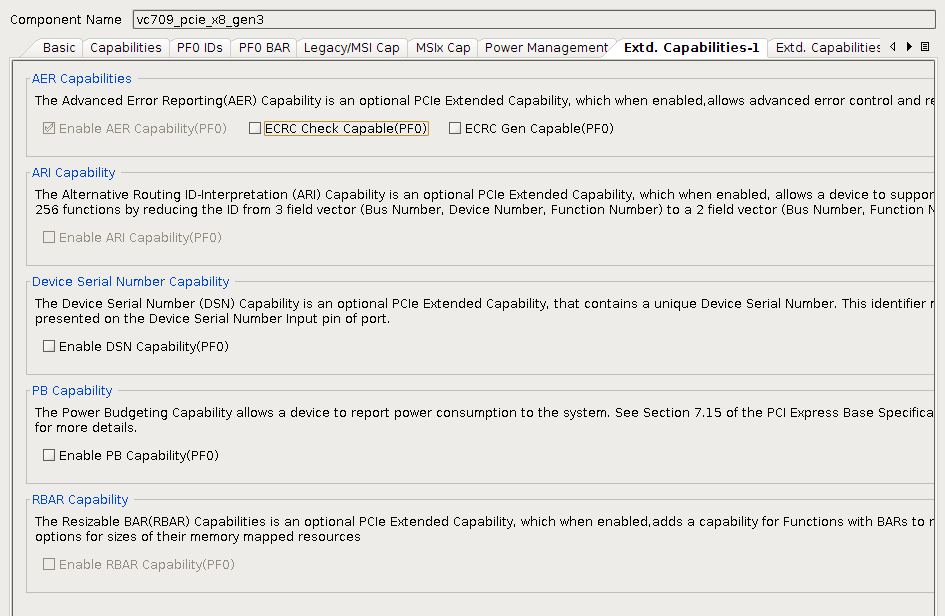
\includegraphics[width=0.75\textwidth]{pictures/pcie_core_extcapa1.png}
\caption{PCIe core configuration in Vivado [Extd. Capabilities 1]}
\label{fig:pcie_core_config8}
\end{figure}
\newpage
\begin{figure}[H]
\centering
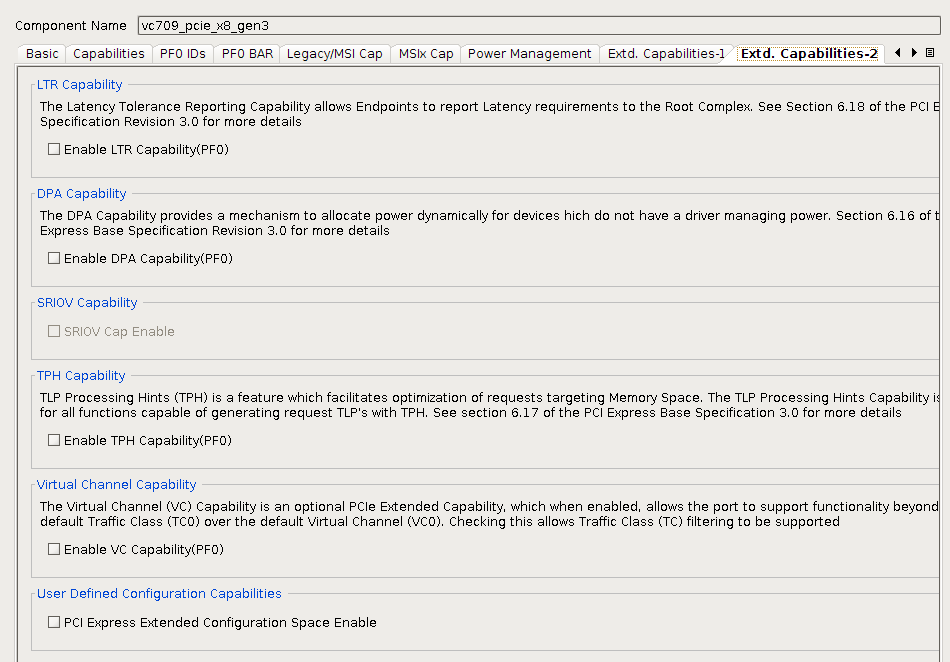
\includegraphics[width=0.75\textwidth]{pictures/pcie_core_extcapa2.png}
\caption{PCIe core configuration in Vivado [Extd. Capabilities 2]}
\label{fig:pcie_core_config9}
\end{figure}


\begin{figure}[H]
\centering
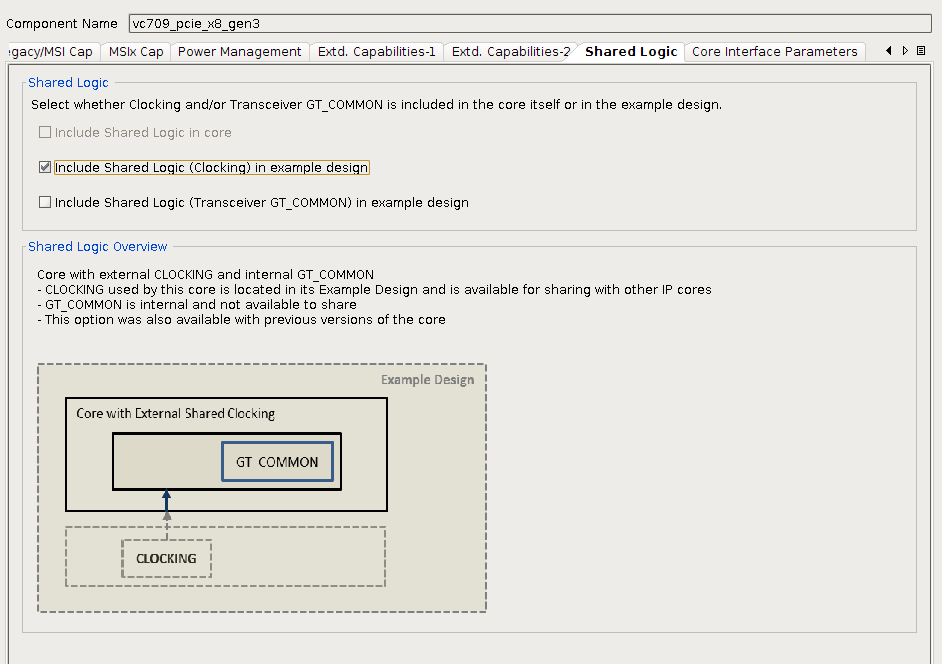
\includegraphics[width=0.75\textwidth]{pictures/pcie_core_shared.png}
\caption{PCIe core configuration in Vivado [Shared LogicMSIx]}
\label{fig:pcie_core_config10}
\end{figure}
\newpage
\begin{figure}[H]
\centering
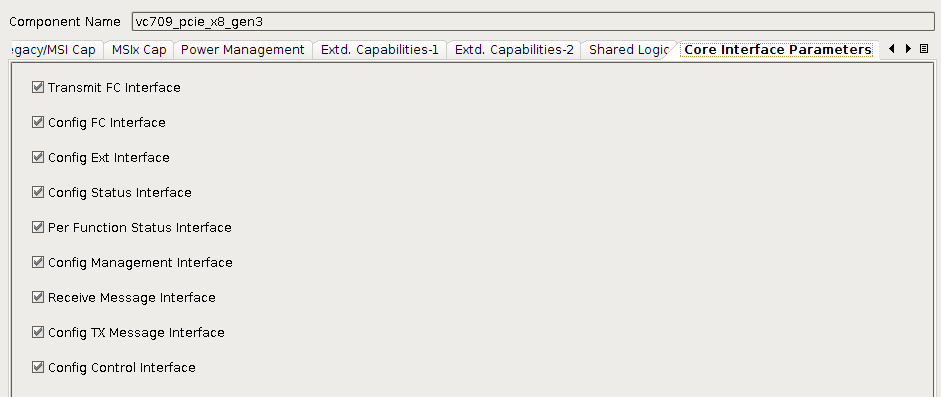
\includegraphics[width=0.75\textwidth]{pictures/pcie_core_coreintpar.png}
\caption{PCIe core configuration in Vivado [Core Interface Parameters]}
\label{fig:pcie_core_config11}
\end{figure}
\newpage